\documentclass[9pt]{beamer}

\geometry{paperwidth=213.3mm,paperheight=120mm}

\usetheme[{titleformat plain}=smallcaps,
           titleformat title=smallcaps,
           titleformat subtitle=regular,
           titleformat section=smallcaps,
           titleformat frame=smallcaps,
           % numbering=fraction,
          ]{metropolis}
% \usepackage{appendixnumberbeamer}

\definecolor{mLightGreen}{HTML}{14B03D}
\definecolor{vpGreen}{HTML}{66c2a5}
\definecolor{vpOrange}{HTML}{fc8d62}
\providecommand{\iRef}[1]{{\color{mLightGreen}\small $[$#1$]$}}

\usepackage{booktabs}
\usepackage[scale=2]{ccicons}

\usepackage{../_style/common}
\usepackage{../_style/defs}

\usepackage{tikz}
\usetikzlibrary{shapes,arrows}
\usepackage{amsmath, bm}
\usepackage{siunitx}
\usepackage{physics,hepnames}
\usepackage{mathtools}
\usepackage{enumitem}
\setenumerate[1]{%
      label=\protect\usebeamerfont{enumerate item}%
      \protect\usebeamercolor[fg]{enumerate item}%
      \insertenumlabel.}
\setitemize{label=\usebeamerfont*{itemize item}%
    \usebeamercolor[fg]{itemize item}
      \usebeamertemplate{itemize item}}

\usepackage{subfig}
\usepackage{colortbl}
\usepackage{multirow}
\usepackage{pifont}

\usepackage{pgfplots}
\usepgfplotslibrary{dateplot}

\usepackage{ulem}

\graphicspath{{pictures/}}

\title{PDF sampling}
\subtitle{as \sout{Bayesian} na\"ive as possible}
\date{August, 2022}
\author{\textit{\textbf{Alessandro Candido}}, Luigi Del Debbio, Tommaso Giani, Giacomo Petrillo}
%\institute{N3PDF}
\titlegraphic{
    \raisebox{10pt}[0pt][0pt]{\includegraphics[width=2.5cm]{../_logos/nnpdf_logo.pdf}}\hspace*{10pt}
    \hfill
    \raisebox{5pt}[0pt][0pt]{\includegraphics[height=0.8cm]{../_logos/n3pdf_logo.pdf}}\hspace*{10pt}
    \includegraphics[height=1.3cm]{../_logos/erc_logo1.png}

    \vfill\vspace*{230pt}
    \includegraphics[height=1cm]{../_logos/unimi_logo.png}\hfill
    \includegraphics[height=1cm]{../_logos/infn_logo.png}\\
    \vspace*{5pt}
    {
        \fontsize{3pt}{3.5pt}\selectfont
        \begin{center}
            This project has received funding from the European Union's Horizon
            2020 research and innovation programme under grant agreement No
            740006\quad \includegraphics[height=5pt]{../_logos/eu-flag.jpg}
        \end{center}
    }
}

\begin{document}

\maketitle

\setlist[description]{font=\quad\normalfont\bfseries\scshape\space}
\metroset{block=fill}

\section{Fitting functions 101}

\begin{frame}{Function space}
    \begin{columns}
        \begin{column}{0.5\textwidth}
            A function $f: \mathbb{R} \to \mathbb{R}$ (or suitable intervals)
            lives in a infinite-dimensional space.
            \vspace*{20pt}

            This has a simple consequence:
            \begin{block}{Under-determination}
                Fitting an \textbf{unknown function} on a finite number of data
                is always an \textbf{under-determined} problem.
            \end{block}
            \vspace*{20pt}

            How to choose a solution, when \alert{many} are available and
            \alert{equivalent}?
        \end{column}
        \begin{column}{0.5\textwidth}
            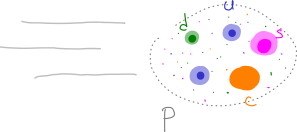
\includegraphics[width=\textwidth]{intrinsic}
        \end{column}
    \end{columns}
\end{frame}

\begin{frame}[standout]
    Let's discuss!
\end{frame}

\end{document}
